\begin{theo}[Elektrische potentiële energie]{Elektrische potentiële energie}

Om de wet van behoud van energie toe te mogen passen, moeten we nog \textbf{elektrische potentiële energie} definiëren. 

% We weten uit hoofdstuk 8:

% \begin{equation*}
%     \Delta U = U_b - U_a = \int_a^b dU = -\int_a^b \Vec{F} \cdot d\Vec{r} = -W
% \end{equation*}

% \noindent Dit kunnen we nu toepassen in de context van de elektrostatische kracht, vermits deze conservatief is:

\begin{equation*}
    \hspace{3.25cm}
    \Delta U = -\int_a^b \Vec{F_e} \cdot d\Vec{r} = -q \int_a^b \Vec{E} \cdot d\Vec{r} = -W \quad \quad (\text{met $q$ een testlading})
\end{equation*}

\noindent In overeenkomst met de wet van behoud van energie, wordt nu elektrische potentiele energie getransformeerd naar kinetische energie. 

\end{theo}

\begin{theo}[Elektrische potentiaal en potentiaalverschil]{Elektrische potentiaal en potentiaalverschil}

    Het \textbf{elektrische potentiaal} $ V $ is een \textbf{scalaire} grootheid die gedefinieerd wordt door het elektrische potentiële energie per lading. In formulevorm:
    
    \begin{equation*}
        V = \dfrac{U}{q}
    \end{equation*}
    
    \noindent Het maakt niet per se uit hoeveel potentiële energie een systeem heeft op een bepaald moment, maar wel hoeveel er naar kinetische energie wordt omgezet. Dus: enkel verschillen in potentiële energie zijn zinvol of betekenisvol. In formulevorm:
    
    \begin{equation*}
         \Delta V = \dfrac{\Delta U}{q} = \dfrac{-W}{q}
    \end{equation*}
    
    \noindent Dit noemt men het \textbf{potentiaalverschil}. De eenheid van eletrische potentiaal, en dus potentiaalverschil, noemt men de volt: $ V = \dfrac{J}{C} $. \\
    
    \noindent Als we de formule van de elektrische potentiele energie in functie van het potentiaalverschil schrijven, dan krijgen we:
    
    \begin{equation*}
        \Delta V  = -\dfrac{1}{q} \int_a^b \Vec{F_e} \cdot d\Vec{r} = -\int_a^b \Vec{E} \cdot d\Vec{r} 
    \end{equation*}
    
    \noindent Dit toont een belangrijk verband aan tussen het elektrische potentiaal en elektrisch veld. Als het veld uniform is, dan hebben de elektrisch veld en de verplaatsing vectoren dezelfde richting en volgt:
    \begin{equation*}
        \Delta V  = -\int_a^b \Vec{E} \cdot d\Vec{r} = - E \int_a^b dr = -Er
    \end{equation*}
    
\end{theo}

\begin{theo}[Equipotentiaaloppervlakken]{Equipotentiaaloppervlakken}

    \textbf{Equipotentiaaloppervlakken} zijn oppervlakken die punten met een equivalent potentiaal verbinden en die loodrecht staan  op de veldlijnen, want de potentiaal moet doorheen het oppervlak gelijk zijn.
    
\end{theo}

\begin{app}[Elektrische potentiaal tegenover puntladingen]{Elektrische potentiaal tegenover puntladingen}

    We hebben eerder besproken dat enkel het potentiaalverschil zinvol is. We kunnen dus een punt pakken waar het potentiaal 0 is en hiermee kunnen we het potentiaal van een singuliere puntlading berekenen. We weten ook dat het elektrisch veld door een singuliere puntlading de volgende formule heeft:
    
    \begin{equation*}
        \Vec{E} = \dfrac{\Vec{F}_e}{q_0}= k_e\dfrac{q}{r^2}\hat{r}
    \end{equation*}
    
    
    \noindent Stel nu dat $ V_b = 0 $ en $ r_b = \infty $ en we een recht pad volgen van $ a \to b $:
    
    \begin{equation*}
        V_a = - \int_a^b \Vec{E} \cdot d\Vec{r} = - E \int_a^{b} dr = - \dfrac{1}{4\pi\epsilon_0}(\dfrac{q}{r_b} - \dfrac{q}{r_a})  = \dfrac{1}{4\pi\epsilon_0}\dfrac{q}{r_a}
    \end{equation*}
    
    \noindent Het elektrische potentiaal is een \textbf{scalar}, dus we kunnen meerdere potentialen gewoon optellen zonder rekening te moeten houden met richting.
    
    \begin{equation*}
        V_{tot} = \sum_i V_{i}= k(\sum_i \dfrac{q_i}{r_{i}})
    \end{equation*}
    
    \noindent We kunnen het concept van meerdere puntladingen verbreden tot infinitesimale puntladingen als we spreken over een continue ladingsverdeling. Zoals vaker volgt nu de volgende formule:
    
    \begin{equation*}
        V = \dfrac{1}{4\pi\epsilon_0}\int\dfrac{dq}{r}
    \end{equation*}
    
    \noindent In principe geeft deze formule ook het volgende:
    
    \begin{equation*}
        dV = -\Vec{E} \cdot d\Vec{s}
    \end{equation*}
    
    \noindent \textbf{Opmerking:} het elektrisch veld in bijvoorbeeld de x-richting is dus gelijk aan $ E_x = -\dfrac{dV}{dx} $ Hieruit kunnen we de volgende formule afleiden:
    
    \begin{equation*}
        \Vec{E} = (-\nabla V)\hat{r} = -\dfrac{dV}{dx}\hat{i} -\dfrac{dV}{dy}\hat{j} -\dfrac{dV}{dz}\hat{k}
    \end{equation*}

\end{app}

\begin{app}[Elektrische potentiaal bij een dipool]{Elektrische potentiaal bij een dipool}

    \begin{minipage}{.68 \textwidth}
        \vspace{-0.4cm}
        Het elektrische potentiaal op een arbitrair punt P wordt gegeven door de volgende formule waarbij $ V = 0 \ op \ r = \infty $:
        
        \begin{equation*}
            V = k\dfrac{q}{r} + k \dfrac{(-q)}{r + \Delta r} = kq(\dfrac{1}{r} - \dfrac{1}{r+ \Delta r}) = kq\dfrac{\Delta r}{r(r+\Delta r)}
        \end{equation*}
        
        \noindent Deze vergelijking wordt vele malen eenvoudiger als we een punt P pakken veel verder weg dan de scheiding tussen de twee ladingen. We zien op de tekening dat: $ \Delta r \approx \ell\cos(\theta) $. Als we nu dus $ r \gg \ell $ pakken, dan is dus $ r \gg \Delta r $ en verandert onze formule:
        
        \begin{equation*}
            V = k\dfrac{q\ell\cos(\theta)}{r^2} = k\dfrac{p\cos(\theta)}{r^2} \quad \quad (r \gg \ell)
        \end{equation*}
        
        % Als we nu herinneren dat het dipoolmoment $ p = Q\ell $, dan krijgen we de volgende formule:
        
        % \begin{equation*}
        %     V = k\dfrac{p\cos(\theta)}{r^2} \quad \quad (r \gg \ell)
        % \end{equation*}
    
    \end{minipage} 
    \begin{minipage}{.28\textwidth}
        \vspace{-0.3cm}
        \begin{center}
            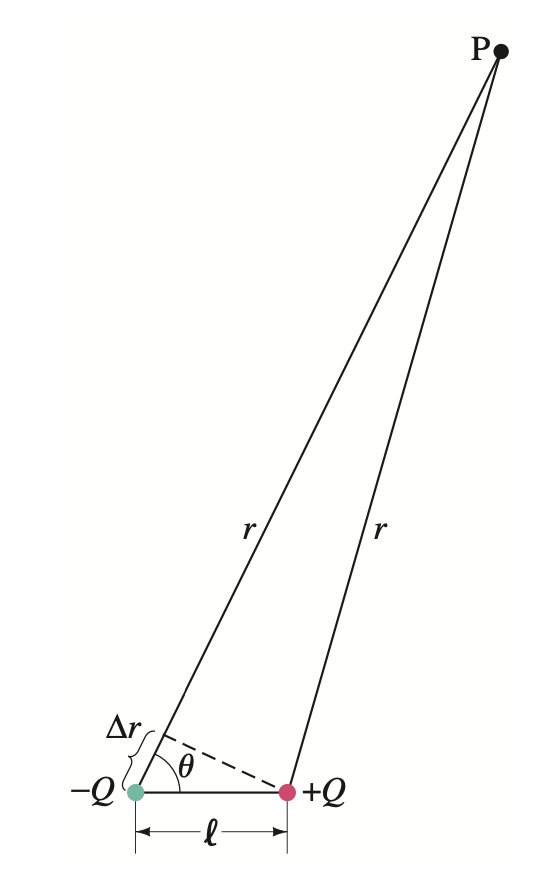
\includegraphics[scale = 0.4]{Images/Elektriciteit/DipoolPotentiaal.png}
        \end{center}
    \end{minipage}

    % \noindent De volgende tekening toont de equipotentiaaloppervlakken aan van een dipool:
    
    % \begin{center}
    %     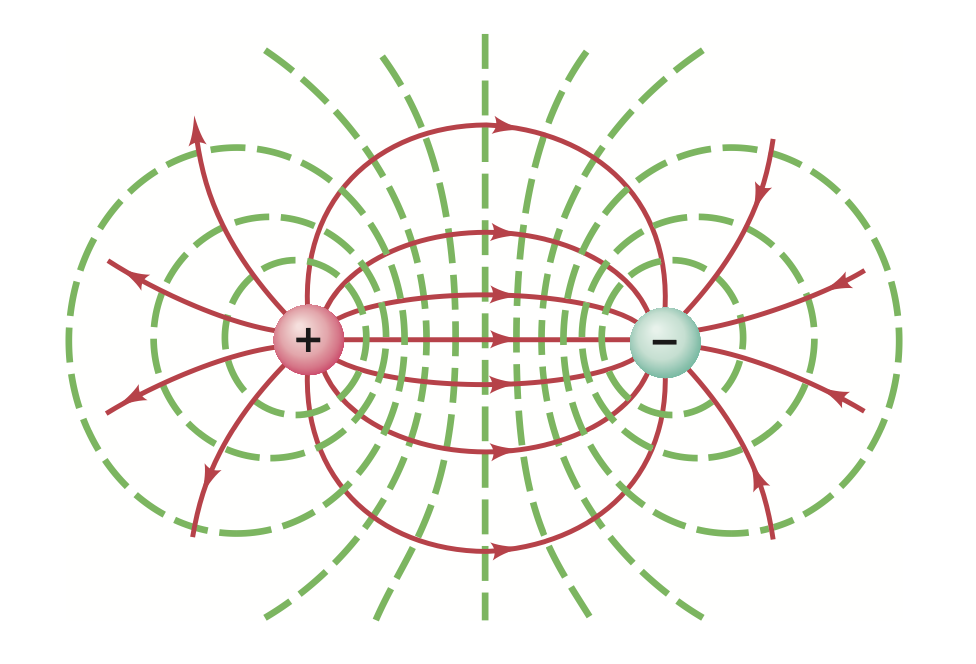
\includegraphics[scale = 0.45]{Images/Elektriciteit/DipoolEquipotentiaaloppervlakken.png}
    % \end{center}
\end{app}

\newpage

\begin{app}[Elektrische potentiaal bij een geladen geleider in evenwicht]{Elektrische potentiaal bij een geladen geleider in evenwicht}

    \begin{itemize}
        \item{\underline{Binnen de geleider zonder caviteit}:} \\
        
        We weten dat het elektrisch veld in de geleider nul is als de geleider zich in een elektrostatisch evenwicht bevindt. We berekenen nu het potentiaalverschil:
        
        \begin{equation*}
            \Delta V = \dfrac{\Delta U}{q} = - \int_a^b \Vec{E} \cdot d\Vec{\ell} = 0
        \end{equation*}
                
        \noindent We kunnen nu bepaalde uitspraken doen over het potentiaalverschil bij een geleider in elektrostatisch evenwicht:
        
        \begin{itemize}
            \item Het oppervlak van een geleider in elektrostatisch evenwicht heeft een constante potentiaal.
            \item  De potentiaal binnenin een geleider is constant, en gelijk aan de potentiaal aan het oppervlak. Er is dus \textbf{geen arbeid} vereist om een lading te bewegen binnenin een geleider
        \end{itemize}
        
        \item{\underline{Binnen de geleider met caviteit}:}
        
        \begin{minipage}{.48\textwidth}
        Het veld in een caviteit (waarbinnen zich geen lading bevindt) omgeven door een geleider is nul. Als er wel een lading in zit, dan moet er aan de rand een gelijke tegengestelde lading zijn opdat er geen elektrisch veld buiten de caviteit zou zijn. Binnenin de caviteit is er natuurlijk dan wel een elektrisch veld. Wegens de wet van behoud van lading, moet er een gelijke positieve lading op het oppervlak van de geleider zijn!
        
        \end{minipage} 
        \begin{minipage}{.48\textwidth}
            \centering
            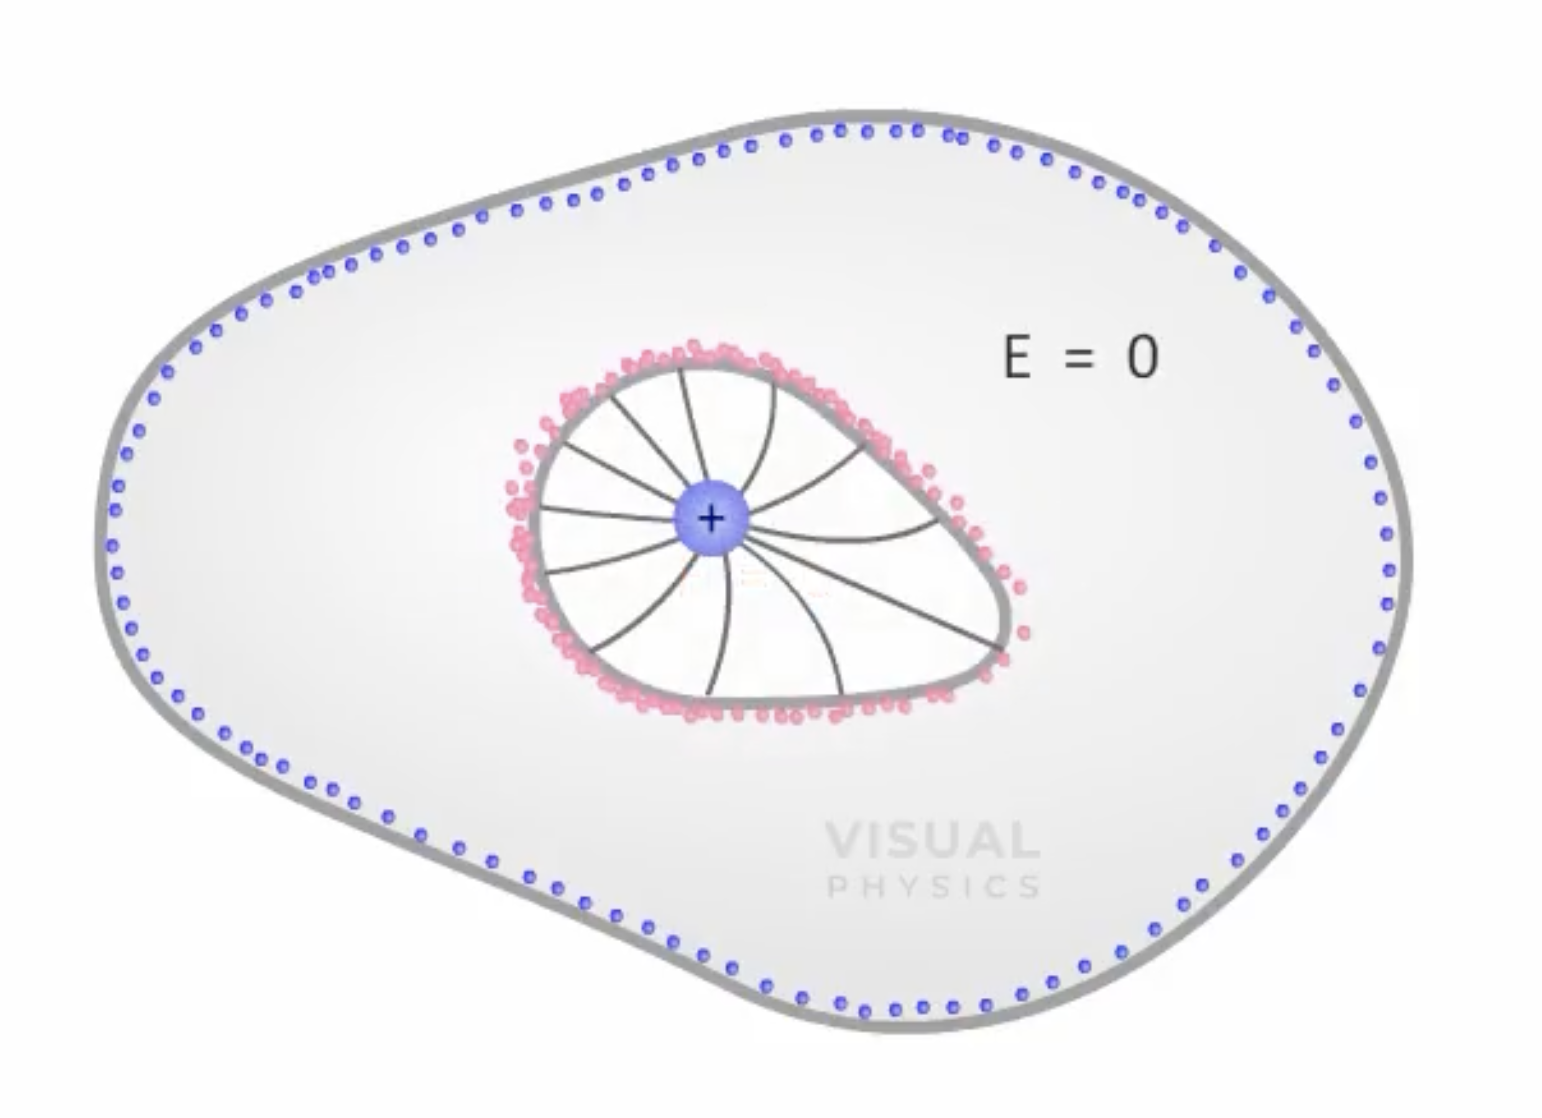
\includegraphics[scale = 0.25]{Images/Elektriciteit/Caviteit.png}
        \end{minipage}
        
        \item{\underline{Buiten de geleider}:} \\
        
        We berekenen het potentiaal van op het oppervlak van een sferische geleider om tot bepaalde conclusies te kunnen komen:
        
        \begin{equation*}
            V = k \dfrac{q}{r} = k \dfrac{\sigma A}{r} = k\dfrac{\sigma 4 \pi r^2}{r} = \dfrac{\sigma r}{\epsilon_0} = Er
        \end{equation*}
        
        \noindent Hieruit volgt dus dat het elektrisch veld groter is nabij convexe punten, vermits het recht evenredig is met de oppervlakteladingsdichtheid. In formulevorm: 
        
        \begin{equation*}
            E \sim \sigma
        \end{equation*}
    
    \end{itemize}
\end{app}

